
El discurso de odio o discriminatorio \footnote{Usaremos de manera indistinta estas expresiones. Para una discusión sobre sus diferencias, ver la sección \ref{sec:hate_speech_definitions}} puede describirse como un discurso en clave de intenso aborrecimiento, denigración y enemistad que ataca a un individuo o un grupo de individuos por poseer --o aparentar poseer-- cierta característica protegida por tratados internacionales como el género, la etnia, la creencia religiosa, el idioma hablado, entre otras. Si bien no hay un consenso generalizado sobre qué configura exactamente discurso de odio \cite{article192015}, un punto de contacto entre las distintas definiciones es su tendencia a generar un ambiente de hostilidad contra grupos o individuos, incitando a la violencia colectiva contra ellos.

En los últimos años, este tipo de discurso ha tomado gran relevancia en redes sociales y otros medios virtuales debido a su intensidad y a su relación con actos violentos contra miembros de estos grupos. A raíz de esto, estados y organizaciones supranacionales como la Unión Europea han sancionado legislación que insta a las empresas de redes sociales a moderar y eliminar contenido discriminatorio. Para citar un ejemplo, desde 2016 Twitter tiene en sus términos y condiciones:

\begin{displayquote}[Política relativa a las conductas de incitación al odio, Twitter]
    Conductas de incitación al odio: No se permite fomentar la violencia contra otras personas ni atacarlas o amenazarlas directamente por motivo de su raza, origen étnico, nacionalidad, pertenencia a una casta, orientación sexual, género, identidad de género, afiliación religiosa, edad, discapacidad o enfermedad grave. Tampoco permitimos la existencia de cuentas cuyo objetivo principal sea incitar la violencia contra otras personas en función de las categorías antes mencionadas.

    Imágenes y nombres de usuario que incitan al odio: No puedes usar imágenes o símbolos de incitación al odio en la imagen o el encabezado de tu perfil. Tampoco puedes usar tu nombre de usuario, nombre visible o biografía de perfil para participar en comportamientos abusivos, como realizar acosos dirigidos o expresar odio contra una persona, un grupo o una categoría protegida.
\end{displayquote}

La enorme cantidad de texto generado por usuarios en las redes sociales --alrededor de 500M de tweets por día son posteados a nivel mundial-- hace imposible que el análisis de este contenido sea realizado de manera enteramente manual. En este escenario de creciente preocupación que genera la proliferación de este discurso, se hace necesario el desarrollo de herramientas que automaticen la detección de discurso de odio en redes sociales, bien sea para el estudio y monitoreo de estas manifestaciones discriminatorias o bien para la moderación.

Desde el procesamiento de lenguaje natural, la detección de discurso de odio puede entenderse en su forma más básica como un problema de clasificación de texto: dado un texto generado por un usuario, predecir si es o no contenido discriminatorio. Así mismo, puede ser de interés predecir otras características: por ejemplo, si el texto contiene un llamado a la acción violenta, si está dirigido contra un individuo o un grupo, el tipo de característica ofendida, entre otras. Poder identificar estas características puede ayudar a delimitar las formas más peligrosas de este fenómeno, como incitaciones a la violencia contra un grupo o individuo.

%Considerando la detección de discurso de odio dentro del área más abarcativa de clasificación de documentos en dominios sociales, analizamos algunos aspectos generales para tareas relacionadas como el análisis de sentimiento y la detección de emociones, entre otras. En particular, analizamos el desempeño de las técnicas de representación al ser entrenadas en distintos dominios. En general, los modelos de representación son entrenados a partir de textos de dominios “formales”, como pueden ser Wikipedia u otras fuentes similares. En esta tesis analizamos el efecto de generar estas representaciones desde textos informales. Observamos que –desde los word embeddings hasta los modelos pre-entrenados basados en transformers– las representaciones generadas son robustas y mejoran la performance en un conjunto de tareas de clasificación en textos sociales. Sobre los modelos pre-entrenados, estudiamos el impacto de entrenarlos desde cero en textos sociales o efectuar una adaptación sobre este dominio

%Todos los estudios y recursos de esta tesis fueron realizados en español. Como un objetivo secundario, pretendemos mitigar la enorme asimetría de recursos existente en el área del procesamiento del lenguaje natural.


\section{Algunos casos resonantes}

Para hacer énfasis en la necesidad de desarrollar herramientas que puedan ayudar a la detección de contenido discriminatorio, comentamos algunos casos puntuales que han tenido lugar en los últimos años en los cuales han co-ocurrido \footnote{Nótese que utilizamos la palabra co-ocurrir y no causar} picos de discurso de odio en redes sociales --mayormente racista o xenófobo-- con eventos de extrema violencia en la vida real. Aún cuando estos ejemplos relatan escenarios en sus formas más brutales, se ha observado que la mera exposición a este discurso en medios virtuales genera un profundo impacto negativo en la psiquis de sus objetivos \cite{saha2019prevalence}, a la vez que prepara un terreno hostil y de deshumanización contra grupos vulnerados, como inmigrantes, minorías religiosas y sexuales \cite{bilewicz2020hate}, algo que ya ha sido estudiado a lo largo de décadas antes de la aparición de las redes sociales e Internet.


\subsection{Atentados en Charlottesville}

En Agosto del 2017, una gran movilización organizada por varios movimientos de ultraderecha y supremacistas blancos tuvo lugar en la ciudad de Charlottesville, Virginia, Estados Unidos. Esta concentración fue llamada en el medio del intento de universitarios y el movimiento Black Lives Matter (BLM) de remover estatuas de militares conferados pro-esclavitud de la Guerra de Secesión a lo largo de todo el territorio de Estados Unidos. En este caso puntual, se intentaba remover la estatua de Robert Lee ubicada en el campus de la Universidad de Virginia, durante los primeros meses de mandato de Donald Trump.

Numerosos grupos de ultraderecha, neonazis, neo-confederados (entre otros) convocaron a la marcha ``Unite the Right''(UtR) para no permitir que se elimine la estatua de Robert Lee, organizando esta marcha como una campaña militar durante varios meses antes de su concreción. \citet{blout2020white} describen la experiencia de Charlottesville como la de un ``terrorismo inmersivo'' ya que generaron un ámbito de terror en varios ``teatros'' (como lo llaman los autores, usando jerga militar). Principalmente, el teatro físico, con la marcha y enfrentamientos con las contra-movilizaciones, la intimidante marcha de antorchas, y el asesinato de Heather Heyer atropellada por un manifestante neo-nazi. Paralelamente, el teatro ``virtual'' situado en las redes sociales sirvió para generar un clima de intimidación antes, durante, y luego del evento mencionado, desplegando --entre otras consignas de carácter racista y xenófobo-- una campaña antisemita contra el alcalde de Charlottesville, de ascendencia judía, y el vicemayor, de ascendencia afroamericana.

\citet{blout2020white} llegan a la conclusión de que el evento fue organizado de manera centralizada, tanto en su planificación como despliegue en un intento de ejercicio militar. También concluyen que la propaganda y la información diseminada por los organizadores sirvió para publicitar y reclutar a simpatizantes como también para aterrorizar a la población de Charlottesville. Esta propaganda se difundió tanto por medios impresos (por ejemplo, posters pegados en las calles) como por redes sociales como Facebook, Twitter o Discord. \citet{klein2019twitter} analiza los intercambios en Twitter entre los dos bandos (manifestantes de ultraderecha y los contramanifestantes) y muestra que, en el caso de quienes se encontraban del lado de la marcha de UtR se identifica como enemigos a los musulmanes, liberales o izquierdistas, a miembros de la comunidad LGBTI \footnote{Lesbianas, Gays, Bisexuales, Transexuales, Intersexuales. Diversas variantes de estas siglas agregan más identidades a este colectivo, como LGBTIQ+.}, judíos, entre otros, dando cuenta del sesgo discriminatorio de este grupo.


\subsection{Matanza en Sinagoga de Pittsburgh}


\begin{figure}[t]
    \centering
    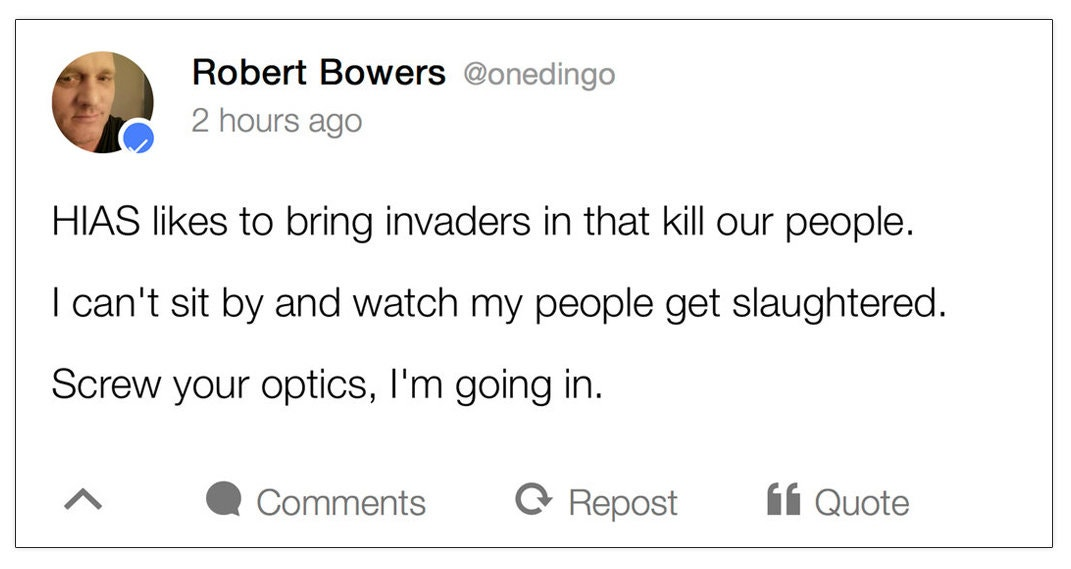
\includegraphics[height=6cm, keepaspectratio]{img/gab-pittsburgh-post.jpg}
    \caption{Último post de Robert Bowers, tirador en la masacre de Pittsburgh, en la red social Gab.}
    \label{fig:gab_post}
\end{figure}


En Octubre de 2018, un hombre fuertemente armado entró a la sinagoga ``El Árbol de la Vida'' en Pittsburgh, Pensilvania, Estados Unidos. Luego de gritar ``muerte a los judíos'', abrió fuego contra la multitud matando 11 personas y dejando decenas de heridos, la matanza más grande de judíos en EEUU de la que se tenga registro.

El tirador, Richard Bowers, era usuario activo de Gab \footnote{\url{https://gab.com/}}, una red social que nació en 2016 bajo la égida de la defensa de la ``libertad de expresión'' a raíz de la creciente moderación de Twitter y Facebook a discursos discriminatorios. Desde entonces, ha sido el refugio de activistas de la derecha alternativa, supremacistas raciales, grupos conspiracionistas y otros elementos reaccionarios. El asesino en cuestión posteaba frecuentemente contenido antisemita en dicha red social \cite{mcilroy2019welcome}, particularmente contra la HIAS (Sociedad Hebrea de auxilio de inmigrantes). En su último post en dicha red social, horas antes de la masacre, Bowers posteó una amenaza (ver figura \ref{fig:gab_post}) diciendo que no podía tolerar ver a su gente ser asesinada (por judíos) y que iba a tomar acciones al respecto.

A raíz de esto, Gab --llamada popularmente como el ``Twitter racista''-- estuvo de baja durante cierto tiempo al serle negado alojamiento web debido a este atentado. Desde entonces, diversos trabajos han recopilado y analizado el contenido discriminatorio en esta red social \cite{mcilroy2019welcome,kennedy2018gab}.



\subsection{Masacre Rohingya en Myanmar}
% https://www.quigsclass.com/uploads/7/2/6/8/72681355/5_myanmar_facebook.pdf
%
Entre 2016 y 2017 fue perpetrada una matanza de la etnia Rohingya, un grupo étnico musulmán, en la República de Myanmar (ex Birmania). Cerca de 25 mil personas fueron masacradas y un éxodo de más de 700 mil personas tuvo lugar hacia la lindante Bangladesh, conformando el campamento de refugiados más grande del mundo en la actualidad. La ONU y algunos estados nacionales han calificado lo ocurrido como un ``genocidio'' y como una ``limpieza étnica''.


Si bien el sometimiento de este pueblo tiene lugar hace décadas, en los últimos años tuvo un gran recrudecimiento motorizado desde las altas esferas gubernamentales y militares birmanas, que niegan cualquier estatus legal a la población rohingya. En ese punto, las redes sociales han jugado un rol de difusor y catalizador de incitaciones a la violencia y noticias falsas alrededor de esta etnia. Según un informe solicitado por Facebook acerca de la situación en Myanmar \cite{warofka2018independent}, gran parte de este problema se debe a un déficit en el ``alfabetismo digital''(sic) de la población de este país, que usa casi exclusivamente Internet a través de dicha red social. Enviados de las Naciones Unidas han acusado directamente a Facebook de haber servido como intermediario de discurso de odio a través de su plataforma \footnote{\url{https://www.reuters.com/article/us-myanmar-rohingya-facebook/u-n-investigators-cite-facebook-role-in-myanmar-crisis-idUKKCN1GO2PN}}, y que ha tenido un ``rol determinante'' en este genocidio.

Organizaciones de derechos humanos de ese país han instado a la empresa de Mark Zuckerberg a invertir recursos en el control del discurso de odio, particularmente aquel que insta a la violencia física \cite{irrawaddy2018zuckerberg}. A finales de 2021, un grupo de refugiados rohingya denunció a Facebook por 150 mil millones de dólares \footnote{\url{https://www.bbc.com/news/world-asia-59558090}} por haber promovido la violencia contra esta etnia, luego de que en 2018 responsables de la empresa admitieran que no se hizo lo suficiente para detener la proliferación del discurso xenófobo contra los rohingya en Myanmar.

Este hecho cuenta con una particularidad: apunta a un idioma --el birmano, idioma oficial en Myanmar-- que dispone de pocos recursos en el área del Procesamiento del Lenguaje Natural. La mayoría de los recursos y estudios están dedicados al idioma inglés, ignorando las particularidades de cada idioma y el componente cultural de algunas tareas, como en este caso la detección de discurso de odio. Además, según Reuters, para finales de 2018 Facebook no contaba con ningún empleado en Myanmar \footnote{\url{https://www.reuters.com/investigates/special-report/myanmar-facebook-hate/}} ni tampoco quedaba claro que alguno de sus empleados dedicados a la tarea del monitoreo sea hablante nativo de birmano.


\section{Avances en IA y NLP}

En los últimos 10 años, el área de la Inteligencia Artificial ha sido sacudida por la irrupción de las redes neuronales. Desde el campo de Visión por Computadora, un conjunto de factores han potenciado el éxito de esta técnica de aprendizaje estadístico: datasets de gran tamaño como ImageNet \cite{imagenet2009deng}, la utilización de dispositivos de gran poder de cómputo como las GPUs, y el desarrollo de mejores algoritmos para su entrenamiento (de optimización, funciones de activación, entre otras cosas). Esta combinación posibilitó que las redes neuronales obtengan mejoras considerables en el desempeño de tareas de reconocimiento de imágenes, trasladándose esto a otras áreas como procesamiento de habla, y a todas las áreas de aprendizaje automático en general, con particular foco de aquellos datos no estructurados como imágenes, sonido, y otras señales.

Este boom inicial tuvo su primera repercusión de magnitud en NLP cerca del año 2013 con el desarrollo de los word-embeddings. La técnica de \emph{word2vec} \cite{mikolov2013distributed} permitió generar representaciones de palabras de manera eficiente sobre grandes cantidades de datos no etiquetados. Estas representaciones de las palabras (podemos pensarlas como vectores de largo fijo asignadas a cada token) han sido la ``salsa secreta'' que permitió el éxito de las redes neuronales en NLP, permitiendo una mejora en las tareas de reconocimiento de entidades nombradas (NER), POS tagging, parsing, clasificación de textos, entre otras. Otro componente de este éxito de las redes neuronales ha sido el uso de redes recurrentes como las Long Short-Term memory (LSTM) \cite{hochreiter1997long} o las Gated Recurrent Units (GRU) \cite{cho-etal-2014-learning}, que permiten codificar secuencias de manera autorregresiva. Un caso de éxito particular utilizando estas redes recurrentes ha sido el de la traducción automática mediante la arquitectura sequence-to-sequence (seq2seq) \cite{sutskever2014sequence}. Estas redes permitieron atacar los problemas de aprendizaje de secuencia a secuencia, como la traducción automática o sumarización de texto, reemplazando sistemas realmente complejos y de difícil mantenimiento (como los de Statistical Machine Translation) por diseños más simples y con una muy superior performance.

En 2017, \citet{vaswani2017attention} propusieron una arquitectura que elimina la estructura recurrente: los \emph{Transformers}. Este modelo utiliza únicamente múltiples capas de auto-atención para el problema de traducción automática. Al eliminar los pasos recurrentes, permitió la paralelización del cálculo y el entrenamiento de arquitecturas verdaderamente profundas para el área de NLP, como ya hace tiempo se utilizaban en el área de Visión por Computadora. En conjunto a la aplicación del pre-entrenamiento utilizando la tarea de modelado de lenguaje (que introdujeron \citet{howard-ruder-2018-universal} con ULMFiT, entre otros trabajos) supusieron un cambio rotundo en el modo en que hacemos NLP hoy día: en lugar de entrenar una red neuronal casi desde cero (quizás sólo con una capa de embeddings con pesos iniciales pre-calculados) sólo ajustamos (\emph{fine-tune}) una gran red neuronal pre-entrenada sobre un dataset de entrenamiento con alguna tarea de modelado de lenguaje. \bert{}, GPT y otros personajes de Plaza Sésamo son algunos de los rutilantes nombres en el zoológico de modelos pre-entrenados. Esta nueva forma de atacar los problemas de aprendizaje automático de NLP supusieron un breakthrough en el área, mejorando la performance sensiblemente en benchmarks de tareas como GLUE \cite{wang-etal-2018-glue}, RACE \cite{lai2017race}, entre otras tareas.

Estos avances han permitido atacar numerosas tareas que quizás parecían fuera de alcance para el área de NLP o bien tenían performances relativamente pobres. Una de estas tareas es la detección de discurso de odio en redes sociales. \todo{A esto le falta un poquito de desarrollo}

\subsection{Asimetría de recursos}

Un problema no menor en el área de NLP es la enorme asimetría de recursos entre idiomas. La inmensa mayoría de recursos --tanto en forma de datasets como modelos-- están diseñados para el inglés. Con el advenimiento de los modelos pre-entrenados basados en Transformers, este problema se agravó ya que estos modelos necesitan muchos recursos computacionales para ser generados. Para atacar este problema, es necesario desarrollar recursos y estudios para los distintos idiomas. Citando a la ``Regla de Bender'' \cite{bender2011achieving}:

\begin{quote}
    Do state the name of the language that is being studied, even if it's English. Acknowledging that we are working on a particular language foregrounds the possibility that the techniques may in fact be language specific. Conversely, neglecting to state that the particular data used were in, say, English, gives [a] false veneer of language-independence to the work.
\end{quote}

Si bien el español puede considerarse de los idiomas dentro del grupo de los de ``altos recursos'' \cite{bender2019rule}, aún así la disparidad de recursos al el inglés es abrumadora. En particular, para el área de interés de esta tesis --la detección de discurso de odio--, los recursos son muy escasos y, en la mayoría de los casos, ``réplicas'' de trabajos hechos en inglés.

\section{Detección de discurso}

%
%
% https://docs.google.com/drawings/d/1wy148WBa5f6FcHco9j9u_Xy8LUrmkREL136JVNOea6Y/edit
%
%

\begin{figure}
    \centering
    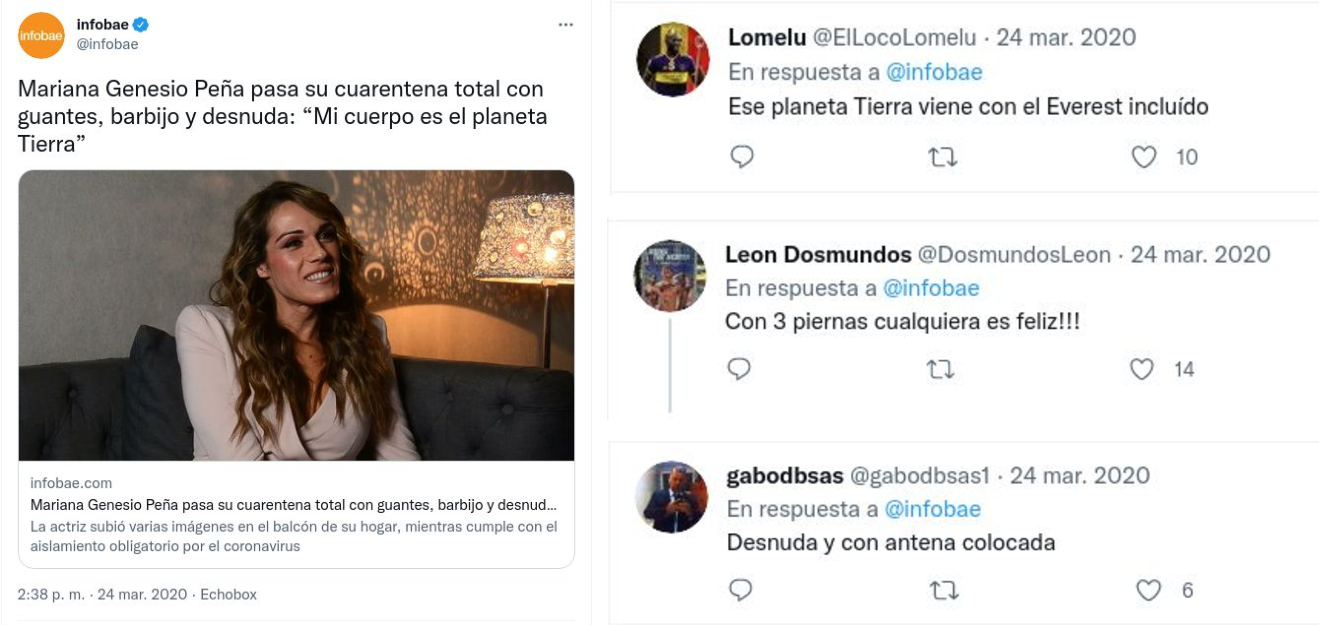
\includegraphics[width=\textwidth]{img/01/tweets_contexto.pdf}
    \caption{Tweets y respuestas discriminatorias. Leyendo únicamente el texto de los comentarios resulta difícil descifrar su sentido. }
    \label{fig:01_tweets_y_su_contexto}
\end{figure}

Como dijimos anteriormente, la detección del discurso de odio puede pensarse como una tarea de clasificación sobre un texto generado por un usuario. Muchos trabajos en los últimos años han abordado la tarea desde esa perspectiva, desarrollándose numerosos recursos en workshops para varios idiomas, y herramientas muy utilizadas para la moderación de contenido tóxico \footnote{El contenido tóxico o abusivo es una categoría un poco más general que la de discurso de odio} como Perspective API \footnote{\url{https://www.perspectiveapi.com/}}, desarrollada por Jigsaw y Google.

Si bien esta este enfoque tiene una innegable utilidad, adolece de ciertas limitaciones. Uno de sus problemas es la falta de contexto en los mensajes analizados. Los seres humanos no solemos recibir mensajes de manera aislada sino que los entendemos a estos situados de acuerdo a varios factores: su emisor, la situación y el medio en el que se lo emite, a quién está dirigido, sobre qué hace mención, entre otras cosas. La mayoría de los estudios y recursos, sin embargo, están hechos sobre datos fuera de contexto: posteos en redes sociales sin ningún tipo de información  conversacional o de otra índole. Para ilustrar el problema de la falta de contexto, la figura \ref{fig:01_tweets_y_su_contexto} muestra un tweet de un medio periodístico que habla sobre una actriz y respuestas a esa noticia \footnote{El hilo completo puede encontrarse en \url{https://twitter.com/infobae/status/1242506130213015552}}. Leyendo los tweets por fuera del contexto es difícil comprender el mensaje y su contenido transfóbico.

La falta de contexto restringe la información disponible --tanto para un humano como para un algoritmo-- para poder discernir si un texto social es discriminatorio. Otra información usualmente faltante y que puede ayudar a enriquecer la detección de discurso de odio es la característica atacada en un texto: es común que los datasets estén anotados de manera poco granular --casi siempre de manera binaria-- no brindando información acerca de si la agresión es por motivos de género, religión, etnia, etc.

Por último, una limitación puntual del español es la poca disponibilidad de recursos para esta tarea, algo que mencionamos en la anterior sección como un problema general de NLP. A este problema se le suma que los pocos datasets disponibles --tanto para español como otros idiomas-- suelen estar generados por anotadores que no son hablantes de las variedades dialectales de los textos utilizados, lo cual genera un déficit en su calidad al ser el lenguaje discriminatorio altamente dependiente de la jerga específica de cada región y de su contexto sociocultural.


\section{Aportes de este trabajo}

En esta tesis nos proponemos hacer un aporte en el sentido de desarrollar mejores mecanismos automáticos de detección de discurso de odio. Si bien el área de NLP ha avanzado enormemente en los últimos años -- y esta subdisciplina en particular ha recibido un gran interés-- creemos que muchos de los enfoques actuales inhiben un avance cualitativo en la detección de este pernicioso fenómeno en medios sociales.

Para ello, en primer lugar estudiamos técnicas de detección sobre datasets ya existentes, utilizando técnicas del estado del arte. En base a la observación de algunos datasets y la literatura en general, plantearemos un nuevo problema: la detección \emph{contextualizada} de discurso de odio. Para ello, construimos un corpus de discurso de odio sobre comentarios en noticias de medios gráficos argentinos en Twitter, siendo este conjunto de datos etiquetado por hablantes nativos. Este dataset es un aporte importante en sí ya que es uno de los primeros datasets que incluyen información contextual, y es el único a nuestro conocimiento en español que tiene esta información. Otras características que lo distinguen es que es uno de los primeros datasets de la variedad dialectal rioplatense a nuestro conocimiento recolectado durante la pandemia de COVID-19.

Con este recurso, exploramos la siguiente pregunta: ¿pueden los métodos actuales basados en modelos pre-entrenados aprovechar información adicional de contexto para mejorar la detección de discurso de odio? Este punto ha sido poco estudiado en la literatura y consideramos que es una pregunta de interés para atravesar los límites de la clasificación basada en una única fuente de información (el comentario analizado). En base a los experimentos realizados, encontramos evidencia que el contexto puede brindar información útil para detectar este fenómeno. Particularmente, observamos que para los mensajes de odio contra ciertos grupos --por ejemplo, contra la comunidad LGBTI-- el contexto puede ser aún más útil para su detección.

Finalmente, realizamos un estudio más en general sobre la \emph{adaptación de dominio} en tareas de clasificación de redes sociales. Para ello, generamos un modelo de lenguaje pre-entrenado sobre textos sociales en español al que bautizamos \robertuito{}, el primero disponible y a gran escala en este idioma. Comparamos la performance de este modelo contra otros modelos pre-entrenados sobre textos formales, y contra modelos ajustados al dominio social. Esta comparación es de interés ya que el ajuste de dominio es relativamente económico frente al enorme costo de entrenamiento que tienen construir modelos como \robertuito{}. Observamos que para todas las tareas, \robertuito{} obtiene una performance del estado del arte, pero el ajuste de dominio recorta considerablemente el gap de performance contra otros modelos.

Un aporte en general de esta tesis es que todos los estudios y recursos han sido realizados en español. Vista la enorme asimetría que hay con otros idiomas, y teniendo en cuenta que el español es el segundo idioma en hablantes nativos del mundo, consideramos necesario mitigar este desbalance de recursos.
